% !TeX spellcheck = en_GB
\def\ChapterTitle{Maritime Communications and Operations}

\chapter{\ChapterTitle}
\label{Chapter\thechapter}
\lhead{Chapter \thechapter.
\emph{\nameref{Chapter\thechapter}}} % Write in your own chapter title to set the page header

\section{Maritime Communications Environment}\label{sec:marine_comms}

The key challenges of underwater acoustic communications are centred around the impact of slow and differential propagation of energy (RF, Optical, Acoustic) through water, and it's interfaces with the seabed / air.
The resultant challenges include; long delays due to propagation, significant inter-symbol interference and Doppler spreading, fast and slow fading due to environmental effects (aquatic flora/fauna; surface weather), carrier-frequency dependent signal attenuation, multipath caused by the medium interfaces at the surface and seabed, variations in propagation speed due to depth dependant effects (salinity, temperature, pressure, gaseous concentrations and bubbling), and subsequent refractive spreading and lensing due to that same propagation variation\cite{Partan2006}.

\subsection{Mechanics of Acoustic Transmission}

Unlike in RF energy transfer (where photons move through space to transmit energy from one place to another), acoustic wages are the result of mechanical perturbation of a medium where localised compressions and extensions pass energy across a medium through that mediums elastic properties.
These ``compression waves'' propagate away from its source, and the rate of this propagation is the sound speed, velocity or $c$, measured in $ms^{-1}$.
This is not to be confused with the fluid velocity corresponding to the instantaneous motion of particles in the medium.

Hydrophones, like their more common microphone equivalent in air, are fundamentally pressure sensors.
Acoustic pressure is usually measured in \emph{Pascals} ($Pa/\mu Pa$). 
In the underwater environment, the dynamic range (difference between instantaneous high and low pressure values) may be extremely high, often more than 10 orders of magnitude higher. 
As such, logarithmic notation is justified.

Useful acoustic signals are generally maintained vibrations rather than instantaneous pulses.
They are characterised by their frequency $f$ expressed in Hertz ($Hz$) or by their Period ($T$) in seconds.
In commonly used underwater acoustics, used frequencies range from $\approx 10Hz-100kHz$ depending on application.\cite{Stojanovic2007}.

As with all waves, the relationship between frequency, period and the wavelength is given as in \eqref{eq:wavelength}. 
As such the generally used upper and lower bounds of wavelength in most applications is from $1.5 m @ 10Hz$ to $0.015m @ 100kHz$.
%
\begin{equation}
  \lambda = cT = \frac{c}{f}
  \label{eq:wavelength}
\end{equation}
%

This wide range of frequencies and wavelengths allow for a diverse set of constraining factors; (Paraphrased from \citet{lurton2010}).

\begin{itemize}
  \item \emph{Attenuation} in water; limiting the maximum usable range, which increases very rapidly with frequency
  \item \emph{Dimensions} of sound source; which increase at lower $f$ for a given transmission power
  \item \emph{Spatial Selectivity} of sources and receivers as $f$ increases, due to similarly increasing directivity of energy propagation.
  \item \emph{Acoustic Response} of target surfaces (analogous to receiver gain in RF networks.
\end{itemize}

\subsection{Velocity and density}

Air has a baseline density of approximately $1.3 kg m^{-3}$, and the speed of sound is typically static around $340 ms^{-1}$.
In sea water, acoustic wave velocity is close to $c=1500ms^{-1}$ (generally between $1450ms^{-1}$ and $1550ms^{-1}$ depending on temperature, pressure, salinity etc.).
Similarly variable is sea water density, which is nominally $\rho = 1030kg m^{-3}$.

While the sea/air surface is (ideally) a simple refractive interface, the interface between open seawater and marine sediment is graduated, with density ranges between $1200 - 2000 kg m^{-3}$. 
This results in refractive and reflective velocities in the sediment interface ranging from $1500-2000 ms^{-1}$\cite{lurton2010}.

For comparison, the speed of light in air/water is $2.99 \times 10^8 ms^{-1}$ and $2.249 \times 10^{8} ms^{-1}$ respectively. 
\todo{this might be better as a table}

\citet{Mackenzie1981} proposed a more accurate model of acoustic velocity incorporating archival data from 15 worldwide sites that takes Temperature, Salinity and Depth into consideration.

\begin{align}
  c = & 1448.96 + 4.591 T - 5.304 \times 10^{-2} T^2 + 2.374 \times 10^{-4}T^{3}\notag\\
  & +1.340 (S-35) + 1.630\times 10^{-2}D+1.675\times 10^{-7}D^2\\
  & -1.025 \times 10^{-2}T(S-25) - 7.139\times 10^{-13}TD^3\notag
  \label{equ:mackenzie}
\end{align}

Where $T$ is the temperature in Celsius, $S$ the salinity in parts per thousand, and $D$ is the depth below the surface in meters.

\todo{Need to discuss Speed of Sound Profiles}

\subsection{Intensity and Power} 

The energy of an acoustic wave is encapsulated into its kinetic and potential parts; where its kinetic energy corresponds to the active motion energy of the particles in the medium, and the potential energy corresponding to the elastic potential of the medium in displacement/compression.

The acoustic intensity ($I$) is the energy flux mean value per unit of surface and time \eqref{eq:acoustic_intensity} in Watts/$m^2$ where $p_0$ is the plane wave amplitude (pressure) and $P_{rms} = p_0/\sqrt{2}$

\begin{equation}
  I = \frac{p_0^2}{2\rho c} = \frac{p_{rms}^2}{\rho c}
  \label{eq:acoustic_intensity}
\end{equation}

\subsection{Attenuation}

The attenuation that occurs in an underwater acoustic channel over a distance $d$ for a signal about frequency $f$ in linear \eqref{eq:acoattenuation} and $dB$ forms \eqref{eq:acoattenuationdb} is given as;

\begin{equation}
  \label{eq:acoattenuation}
  A_{\text{aco}}(d,f) = A_0d^ka(f)^d
\end{equation}
\begin{equation}
  \label{eq:acoattenuationdb}
  10 \log A_{\text{aco}}(d,f)/A_0 = k \cdot 10 \log d + d \cdot 10 \log a(f)
\end{equation}

where $A_0$ is a unit-normalising constant, $k$ is a geometric spreading factor (commonly taken as 1.5 for practical use, but may be 2 for perfect spherical propagation or 1 for perfect plane-wave propagation)), and $a(f)$ is the absorption coefficient, that may be modelled in a variety of ways.

Thorp's formula (\autoref{eq:thorp}) is very simple, only depending on $f$, and is designed to be most accurate about a temperature of 4$^{\circ}$C at a depth of $\approx 1Km$.
%
\begin{figure}
  \begin{equation}
    10 \log a(f) = 0.11 \cdot \frac{f^2}{1+f^2} + 44\cdot\frac{f^2}{4100+f^2}+ 2.75\times10^{-4} f^2 + 0.003
    \label{eq:thorp}
  \end{equation}
  \caption[Thorp's formula]{Thorp's Absorption Model\cite{Stojanovic2007}}
    \label{fig:thorp}
\end{figure}
%
The Ainslie \& McColm model is more complex, and incorporates the acidity of the water ($H^+$) as well as temperature ($T$), salinity ($S$ in parts per trillion) but not depth (\autoref{fig:ainslie}).
%
\begin{figure}
  \begin{align}
    10 \log a(f) =& 0.106 \frac{t_1 f^2}{t_1^2 + f^2} e^{\frac{H^+-8}{0.56}}\\\notag
      & + 0.52 \left(1+\frac{T}{43}\right)\left(\frac{S}{35}\right)\frac{t_2f^2}{t_2^2+f^2} e^{\frac{-D}{6}}\\\notag
      & + 4.9 \times 10^{-4} f^2e^{-\left(\frac{T}{27}+\frac{D}{17}\right)}\\\notag
      \text{Where}&\\\notag
      t_1 =& 0.78 \sqrt{\frac{S}{35}e^{\frac{T}{26}}}\\\notag
      t_2 =& 42 e^{\frac{T}{17}}\notag
      \label{eq:ainslie}
  \end{align}
  \caption{Ainslie \& McColm Absorption Model}
  \label{fig:ainslie}
\end{figure}
%
\begin{figure}
  \begin{align}
    10 \log a(f)=& A_1P_1\frac{t_1f^2}{t_1^2+f^2} + A_2P_2\frac{t_2f^2}{t_2^2+f^2} + A_3P_3f^2\\\notag
    \text{Where }&\\\notag
    A_1=&1.03\times 10^{-8} + 2.36\times 10^{-10} \cdot T -5.22 \times 10^{-12}\cdot T^2\\\notag
    A_2=&5.62\times 10^{-8} + 7.52\times 10^{-10} \cdot T\\\notag
    A_3=&\left(55.9 - 2.39\cdot T + 4.77\times 10^{-2}\cdot T^2 - 3.48 \times 10^{-4}\cdot T^3\right) \times 10 ^{-15}\\\notag
    t_1=&1.32\times 10^3\left(T+273.1\right)e^{\frac{-1700}{T+273.1}}\\\notag
    t_2=&1.55\times 10^7\left(T+273.1\right)e^{\frac{-3052}{T+273.1}}\\\notag
    P_1=&1\\\notag
    P_2=&\-10.3\times 10^{-4}\cdot P + 3.7\times 10^{-7}\cdot P^2\\\notag
    P_3=&\-3.84\times 10^{-4}\cdot P + 7.57\times 10^{-8}\cdot P^2\notag
    \label{eq:fisher}
  \end{align}
  \caption{Fisher-Simmons Absorption Model}
  \label{fig:fisher}
\end{figure}
%
The Fisher-Simmons model (\autoref{fig:fisher}) is significantly more complex, taking into account the effects of boric acid concentrations and dissolved magnesium sulphate. While there are several limitations on this model in terms of its being fixed at a salinity of 35 ppt and a pH of 8, as this model incorporates depth, temperature, distance and frequency, it is very attractive for research directed at high variability environments.\todo{Possibly need to switch this with the Francois Garrison model which, depending on your source, is the refined version (or vise versa}



Regardless of the variations of particular attenuation models, comparing $A_{aco}(d,f)$ with the RF Free-Space Path Loss model $(A_{\text{RF}}(d,f) \approx \left( \frac{4\pi d f}{c} \right)^2)$, the impact of range on signal power is exponential underwater, rather than quadratic in terrestrial RF ($A_{\text{aco}} \propto f^{2d}$ vs $A_{\text{RF}} \propto (df)^2$). 
While both frequency dependant factors are quadratic, approximating the factors in \eqref{eq:thorp}, $f\propto A_{\text{aco}}$ is at least 4 orders of magnitude higher than $f\propto A_{\text{RF}}$
\begin{equation}
  \label{eq:fspl}
  A_{\text{RF}}(d,f) \approx \left( \frac{4\pi d f}{c} \right)^2
  \text{where }c\approx 3\times10^8ms^{-1}
\end{equation}


 \subsection{Ambient Noise Model}

 Ambient ocean noise can be assumed to be Gaussian with a continuous power spectral density in dB re $\mu$Pa per Hz, driven by four major factors, shown in \autoref{tab:ocean_noise_factors}, where $s$ is a shipping activity factor bounded from $[0,1]$ and $w$ is the surface wind speed in $ms^{-1}$ \cite{coates1989}.

\begin{table}\centering
  \caption{Contributing factors to Ocean Ambient Acoustic Noise}
  \label{tab:ocean_noise_factors}
  \begin{tabularx}{\textwidth}{p{3.5cm} X}\toprule
    Source & Approximation \\ \midrule
    Turbulence & $10 \log N_t(f)=17-30\log f$\\
    Shipping & $10 \log N_s(f) = 40+20(s-0.5)+26\log f-60\log(f+0.03)$\\
    Wind Driven Waves & $10\log N_w(f) = 50+7.5w^{\frac{1}{2}}+20\log f - 40\log(f+0.4)$\\ 
    Thermal Noise & $10\log N_{th}(f) = \-15 + 20 log f$\\\bottomrule
  \end{tabularx}
\end{table}

\subsection{Multipath effects}

Refractive lensing and the multi-path nature of the medium result in line of sight propagation being extremely unreliable for estimating distances to targets.
The first arriving acoustic signal has as the very least curved in the medium, and commonly has reflected off the surface/seabed before arriving at a receiver, creating secondary paths that are sometimes many times longer than the first arrival path, generating symbol spreading over orders of seconds depending on the ranges and depths involved.
Thus, the multi-path channel transfer function can be described by 

\begin{align}
  \label{eq:acomultipath}
  H(d,f) =\sum_{p=0}^{P-1} h(p) = \sum_{p=0}^{P-1} \Gamma_p / \sqrt{A(d_p,f)}e^{-j 2 \pi f \tau_p} \\
  \text{where } \tau_p = d_p/c, c \approx 1500 ms^{-1} \notag
\end{align}

where $d=d_0$ is the minimal path length between the transmitter and receiver, $d_p,p=\{1,\dots P-1\}$ are the secondary path lengths, $\Gamma_p$ models additional losses incurred on each path such as reflection losses at the surface interface, and $\tau_p = d_p/c$ is the delay time.

\begin{figure}
  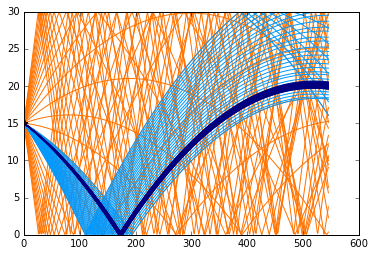
\includegraphics{ghia_sound_prop_curve}
  \caption{Non-Linear Marine Propagation in an isothermal profile}
  \todo[inline]{Vectorise and Label}
  \label{fig:ghia_sound_prop_curve}
\end{figure}



\subsection{Modelling and Simulation of the Acoustic Medium / Channel}

Several toolkits exist in a variety of states that perform communications agent simulation, most notably the NS-2 / 3 family of frameworks and their addons.
Some of these frameworks, such as SUNSET \cite{Petrioli2012a} and AquaTools \cite{Sehgal2010}.

Beyond the NS family, there are many other communications and simulation modelling systems such as OpNet++\cite{Chang1999} and MATLAB toolkits such as the AcTUP interface to the Ocean Acoustics Library.


\todo{expand this, justify AUVNetSim, reactive mobility, python compatibility, SimPy Etc.}


\subsection{Routing and Network Design for \glspl{uan}}

Forward Error Correction coding is used on such channels to minimise packet losses.

\todo{Summary of Akyildiz02/05}

\section{Marine Operations}\label{sec:marine_ops}

\subsection{Typical \gls{auv} mission profiles}

\todo{Typical AUV missions, payloads, and available equipment}

\subsection{Potential Future Applications}
\todo{Future Applications of AUVs}

\subsection{Need for Trust in Maritime Networks}

As \acrfull{auv} platforms become more capable and economical, they are being used in many applications requiring trust.
These applications are using the collective behaviour of teams or fleets of these \glspl{auv} to accomplish tasks \cite{Caiti2011}.
With this use being increasingly isolated from stable communications networks, the establishment of trust between nodes is essential for the reliability and stability of such teams.
As such, the use of trust methods developed in the terrestrial \gls{manet} space must be re-appraised for application within the challenging underwater communications channel.



%%%%%%%%%%%%%%%%%%%%%%%%%%%%%%%%%%%%%%%%%%%%%%%%%%%%%%%%%%%%%%%%%%%%%%%%%%%%%%%
